\PassOptionsToPackage{unicode=true}{hyperref} % options for packages loaded elsewhere
\PassOptionsToPackage{hyphens}{url}
\documentclass[11pt,ignorenonframetext,aspectratio=169]{beamer}
\IfFileExists{pgfpages.sty}{\usepackage{pgfpages}}{}
\setbeamertemplate{caption}[numbered]
\setbeamertemplate{caption label separator}{: }
\setbeamercolor{caption name}{fg=normal text.fg}
\beamertemplatenavigationsymbolsempty
\usepackage{lmodern}
\usepackage{amssymb,amsmath}
\usepackage{ifxetex,ifluatex}
\usepackage{fixltx2e} % provides \textsubscript
\ifnum 0\ifxetex 1\fi\ifluatex 1\fi=0 % if pdftex
  \usepackage[T1]{fontenc}
  \usepackage[utf8]{inputenc}
\else % if luatex or xelatex
  \ifxetex
    \usepackage{mathspec}
  \else
    \usepackage{fontspec}
\fi
\defaultfontfeatures{Ligatures=TeX,Scale=MatchLowercase}







\fi

  \usetheme[]{metropolis}






% use upquote if available, for straight quotes in verbatim environments
\IfFileExists{upquote.sty}{\usepackage{upquote}}{}
% use microtype if available
\IfFileExists{microtype.sty}{%
  \usepackage{microtype}
  \UseMicrotypeSet[protrusion]{basicmath} % disable protrusion for tt fonts
}{}


\newif\ifbibliography


\hypersetup{
      pdftitle={Modes of reproduction and pollination control},
        pdfauthor={Deependra Dhakal},
          pdfborder={0 0 0},
    breaklinks=true}
%\urlstyle{same}  % Use monospace font for urls







% Prevent slide breaks in the middle of a paragraph:
\widowpenalties 1 10000
\raggedbottom

  \AtBeginPart{
    \let\insertpartnumber\relax
    \let\partname\relax
    \frame{\partpage}
  }
  \AtBeginSection{
    \ifbibliography
    \else
      \let\insertsectionnumber\relax
      \let\sectionname\relax
      \frame{\sectionpage}
    \fi
  }
  \AtBeginSubsection{
    \let\insertsubsectionnumber\relax
    \let\subsectionname\relax
    \frame{\subsectionpage}
  }



\setlength{\parindent}{0pt}
\setlength{\parskip}{6pt plus 2pt minus 1pt}
\setlength{\emergencystretch}{3em}  % prevent overfull lines
\providecommand{\tightlist}{%
  \setlength{\itemsep}{0pt}\setlength{\parskip}{0pt}}

  \setcounter{secnumdepth}{0}


  \usepackage{setspace}
  \usepackage{wasysym}
  % \usepackage{fontenc}
  \usepackage{booktabs,siunitx}
  \usepackage{longtable}
  \usepackage{array}
  \usepackage{multirow}
  \usepackage{wrapfig}
  \usepackage{float}
  \usepackage{colortbl}
  \usepackage{pdflscape}
  \usepackage{tabu}
  \usepackage{threeparttable}
  \usepackage{threeparttablex}
  \usepackage[normalem]{ulem}
  \usepackage{makecell}
  \usepackage{xcolor}
  \usepackage{tikz} % required for image opacity change
  \usepackage[absolute,overlay]{textpos} % for text formatting
  \usepackage[skip=0.333\baselineskip]{caption}
  % \usepackage{newtxtext,newtxmath}% better than txfonts   
  \usepackage[english]{babel}
  \usepackage{pgfpages}

  \sisetup{per-mode=symbol}

  % % Added by CII
  % \usepackage[format=hang,labelfont=bf,margin=0.5cm,justification=centering]{caption}
  % \captionsetup{font=small,width=0.9\linewidth,labelfont=small,textfont={small}}
  % % End of CII addition

  % \usepackage{subcaption}
  % \newcommand{\subfloat}[2][need a sub-caption]{\subcaptionbox{#1}{#2}}

  \captionsetup[sub]{font=footnotesize,labelfont=footnotesize,textfont=footnotesize}
  % \captionsetup[subfigure]{font=small,labelfont=small,textfont=small}
  % \captionsetup[subfloat]{font=scriptsize,labelfont=scriptsize,textfont=scriptsize}

  % this font option is amenable for beamer, although these are global settings
  \setbeamerfont{caption}{size=\tiny}
  % \setbeamerfont{subcaption}{size=\tiny} % this does not chage subfloat fonts
  % \setbeamerfont{subfloat}{size=\tiny} % this does not change subfloat fonts
   
   % use single line spacing ?
  \singlespacing

  % use cslreferences environment

  \newlength{\cslhangindent}
  \setlength{\cslhangindent}{1.5em}
  \newenvironment{cslreferences}%
    {\setlength{\parindent}{0pt}%
    \everypar{\setlength{\hangindent}{\cslhangindent}}\ignorespaces}%
    {\par}

  \title[]{Modes of reproduction and pollination control}


  \author[
        Deependra Dhakal
    ]{Deependra Dhakal}

  \institute[
    ]{
    Gokuleshwor Agriculture and Animal Science College\\
Tribhuwan University\\
\textit{ddhakal.rookie@gmail.com}\\
\url{https://rookie.rbind.io}
    }

\date[
      Academic year 2019-2020
  ]{
      Academic year 2019-2020
        }

\begin{document}

% Hide progress bar and footline on titlepage
  \begin{frame}[plain]
  \titlepage
  \end{frame}



\hypertarget{introduction}{%
\section{Introduction}\label{introduction}}

\begin{frame}{}
\protect\hypertarget{section}{}
\begin{figure}

{\centering 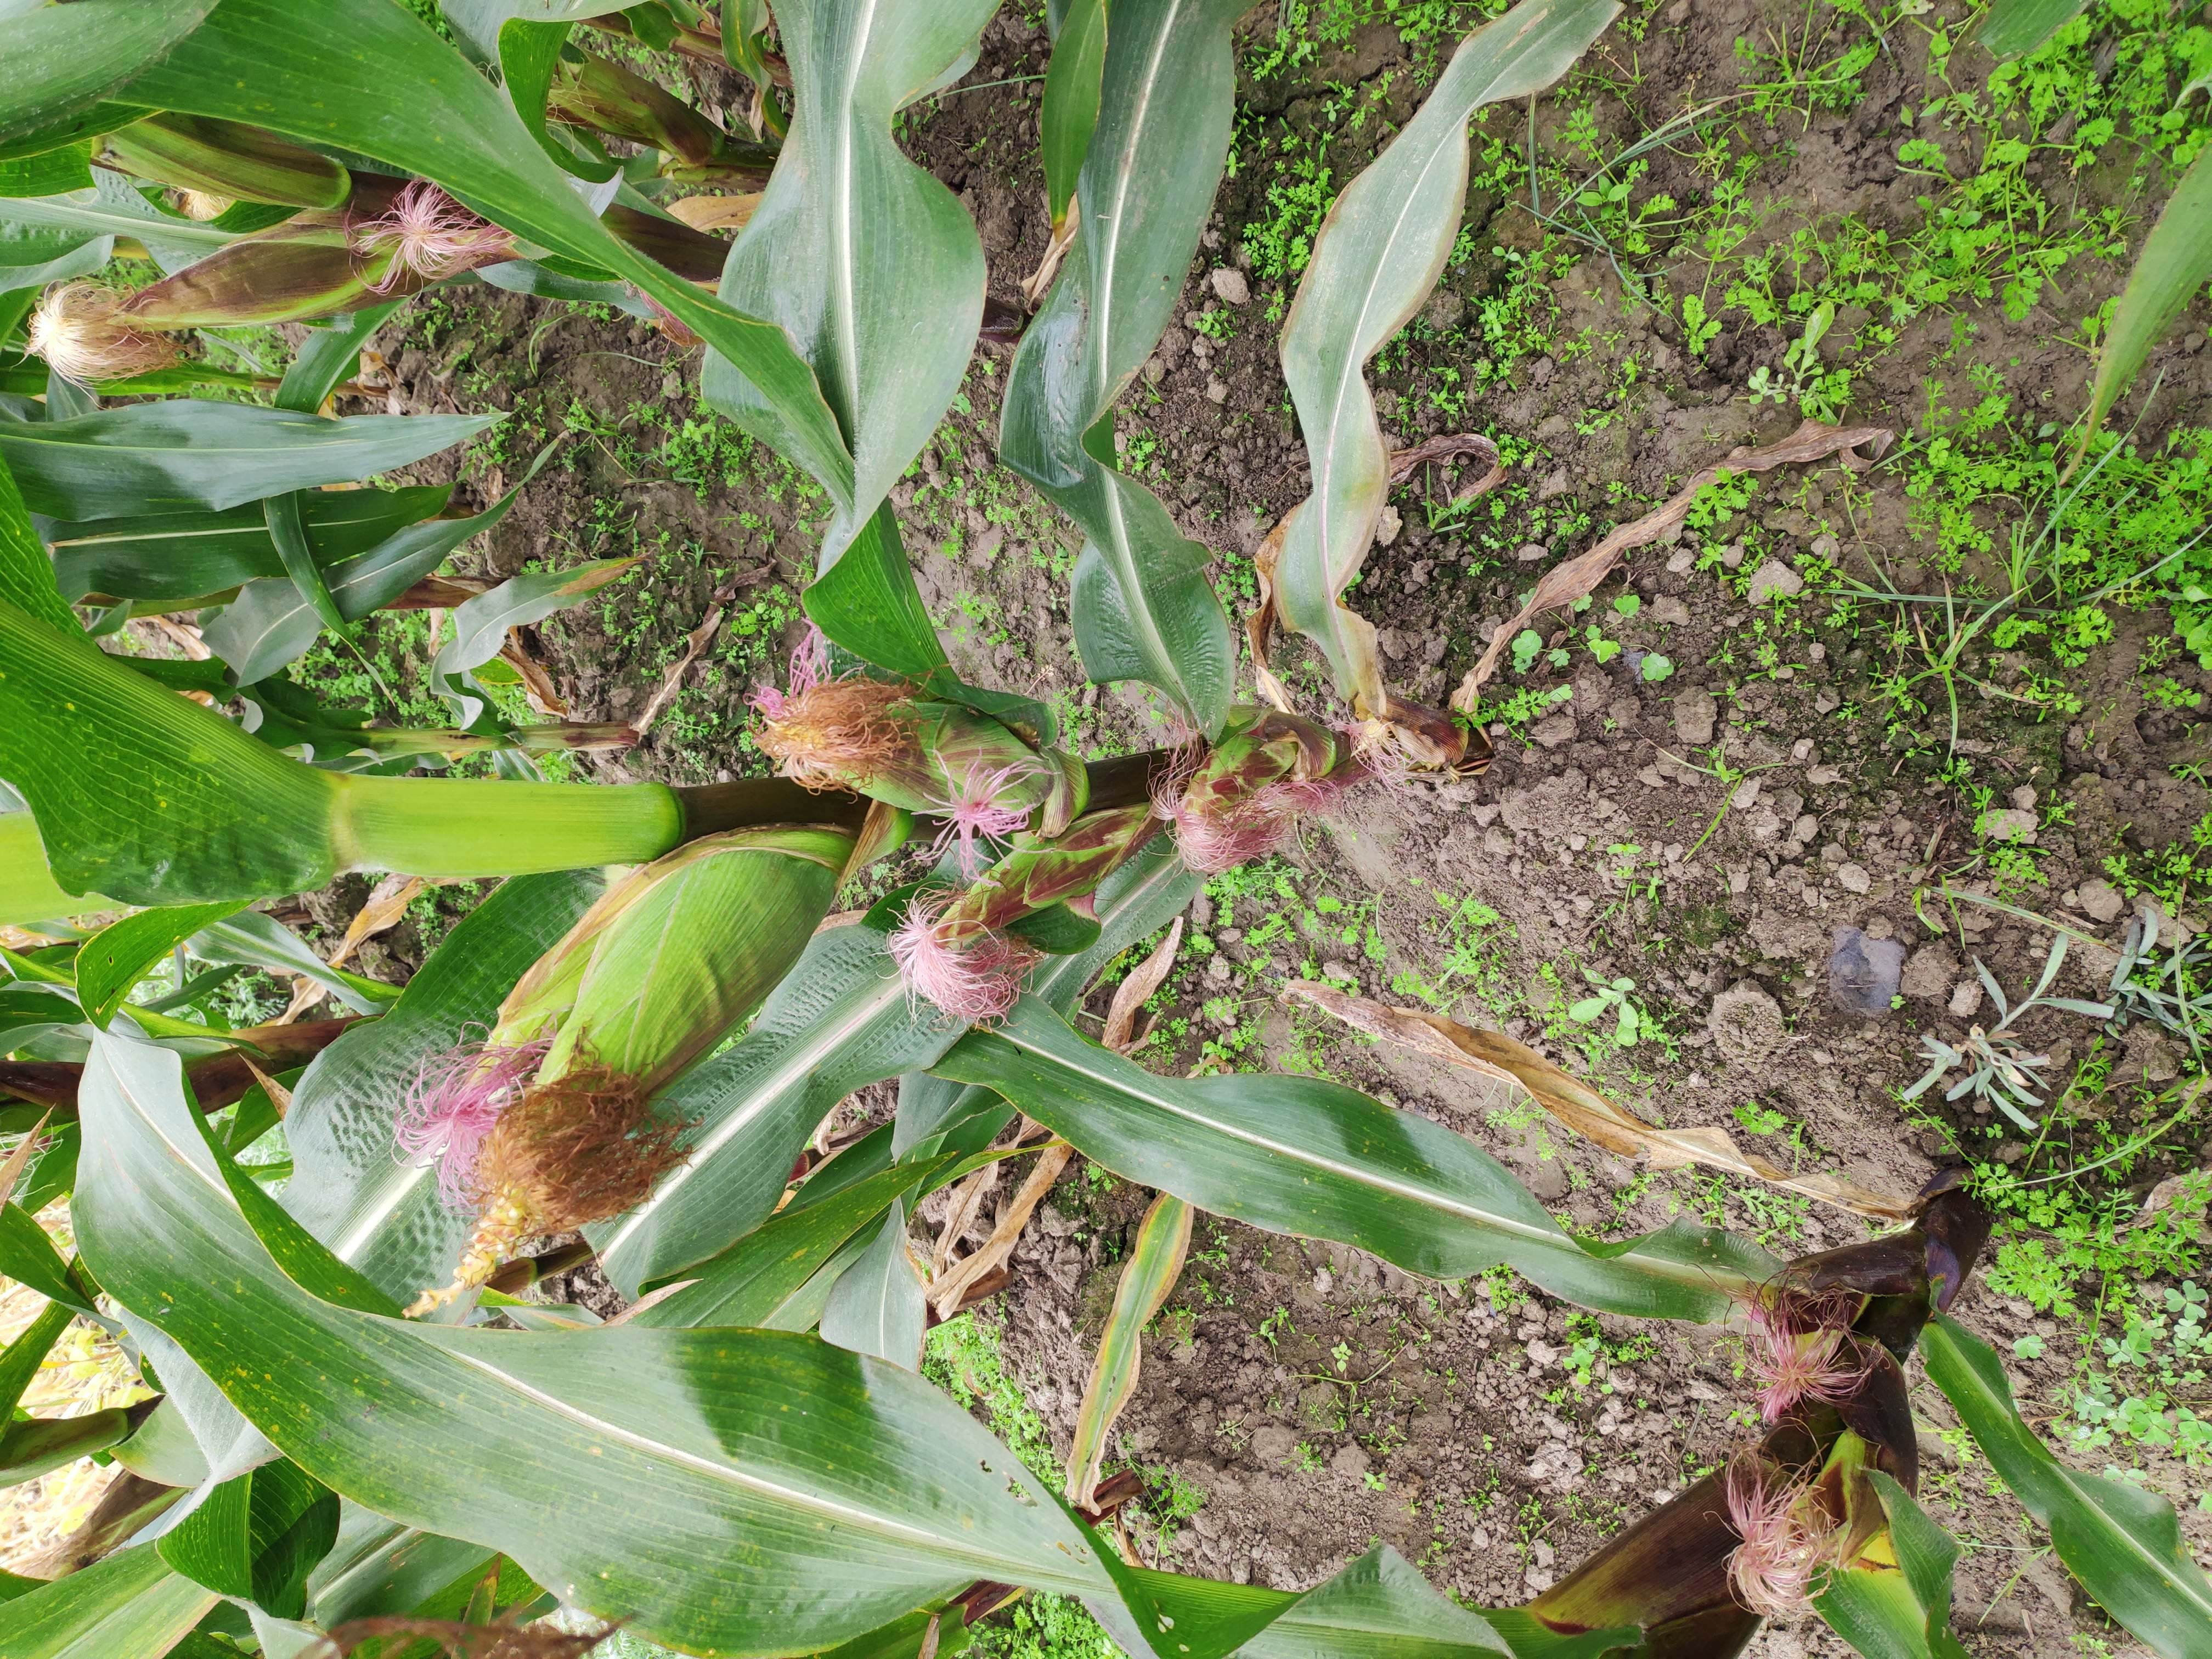
\includegraphics[width=0.7\linewidth]{./images/Maize_inbred} 

}

\caption{Inbred line of maize}\label{fig:maize}
\end{figure}
\end{frame}

\hypertarget{modes-of-reproduction}{%
\section{Modes of reproduction}\label{modes-of-reproduction}}

\begin{frame}{Sexual reproduction}
\protect\hypertarget{sexual-reproduction}{}
\begin{itemize}
\tightlist
\item
  Involves fusion of male and female gametes
\item
  Gametes may be derived either from two different parents or from a
  single parent.
\item
  Sexual reproduction is reliant on the process of meiosis. Involves

  \begin{itemize}
  \tightlist
  \item
    Megaspores within the ovule of the pistil
  \item
    Microspores within the stamen
  \end{itemize}
\item
  Typical meiotic division of a female diploid species will result in
  formation of four haploid megaspores (\emph{Megasporogenesis}).
\item
  With analogy: \emph{Microsporogenesis}
\item
  Hence fertilization involves fusion of haploid male gamete with
  haploid female gamete
\item
  Male gametophyte generation is a tiny pollen tube and three haploid
  nuclei (\emph{microgametophyte})
\item
  Female gametophyte is a single multinucleated cell, also called the
  embryo sac (\emph{megagametophyte}, aka embryo sac).
\end{itemize}
\end{frame}

\begin{frame}{}
\protect\hypertarget{section-1}{}
\begin{figure}

{\centering 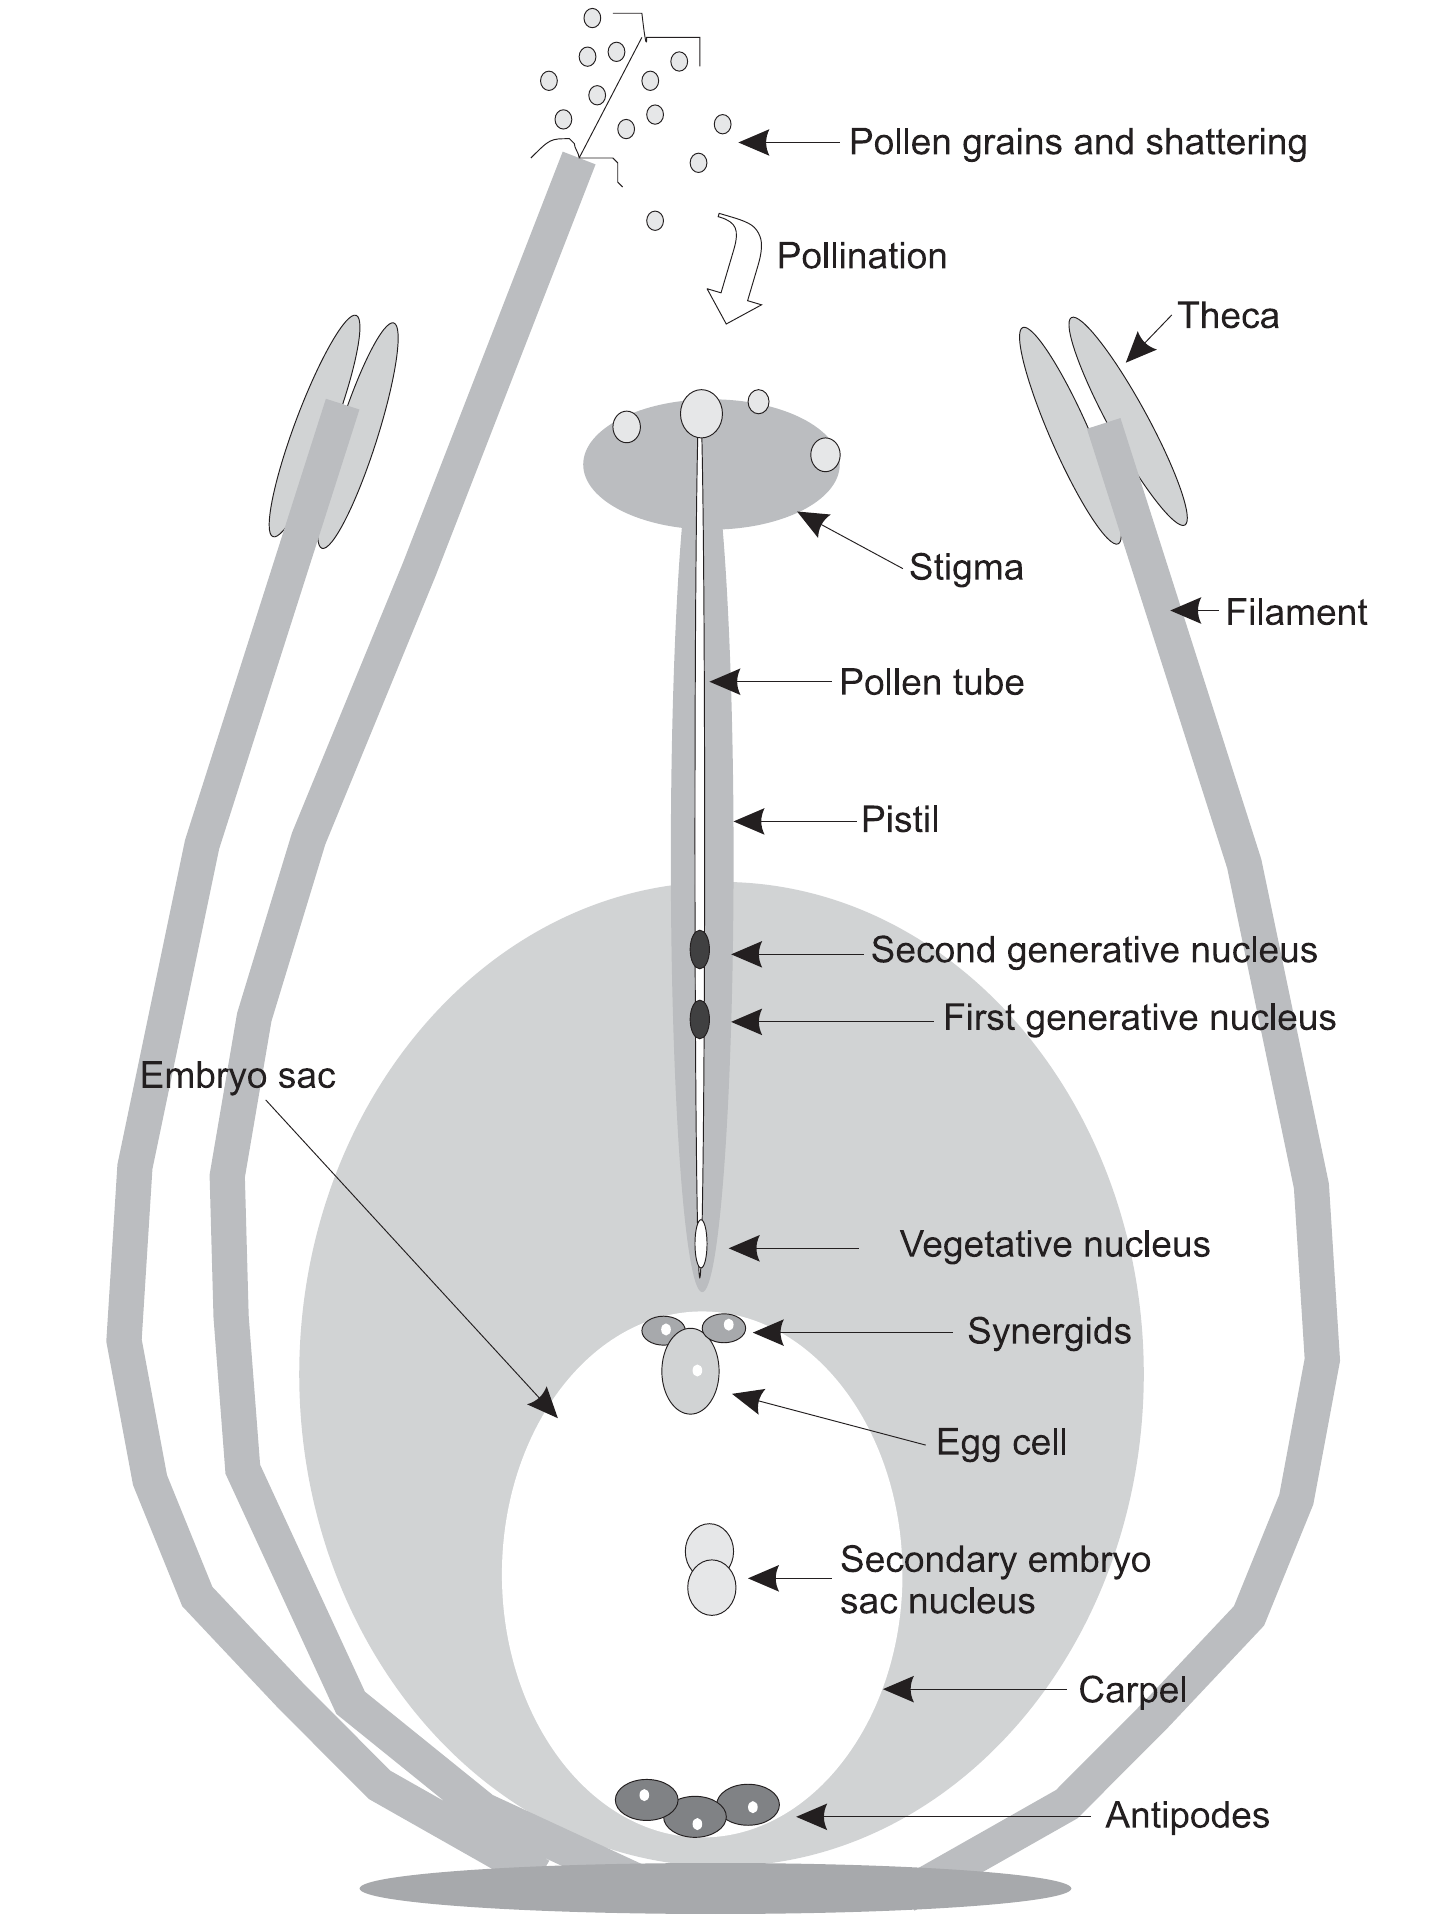
\includegraphics[width=0.38\linewidth]{./images/fertilization_in_self_pollinated_species} 

}

\caption{Fertilization in plants}\label{fig:plant-fertilization}
\end{figure}
\end{frame}

\begin{frame}{}
\protect\hypertarget{section-2}{}
\begin{figure}

{\centering 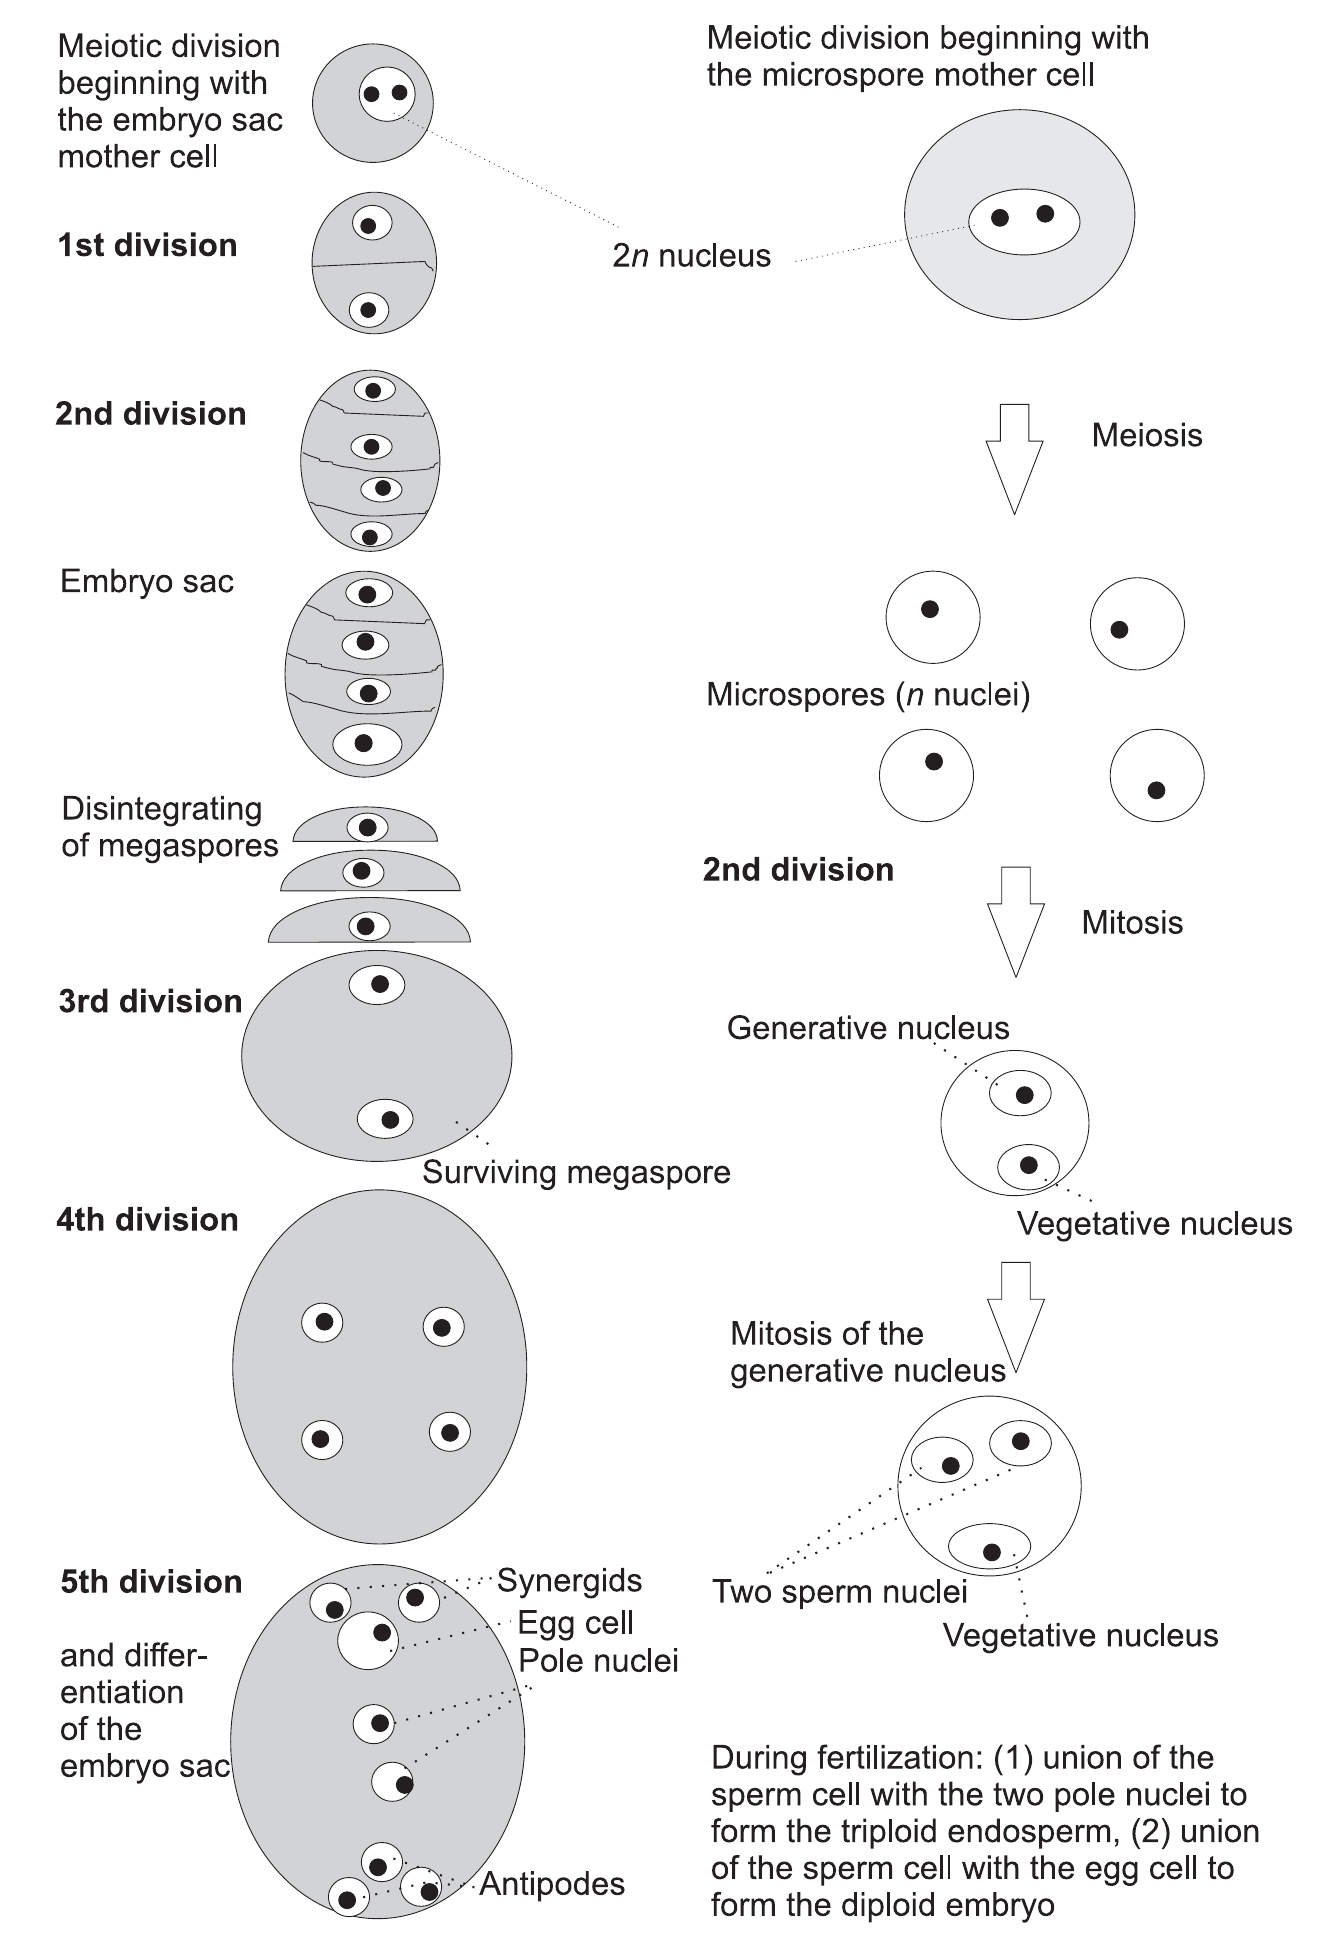
\includegraphics[width=0.38\linewidth]{./images/sporogenesis} 

}

\caption{Embryo sac and pollen formation}\label{fig:sporogenesis}
\end{figure}
\end{frame}

\begin{frame}{Autogamy/Self-pollination}
\protect\hypertarget{autogamyself-pollination}{}
\begin{itemize}
\tightlist
\item
  Mechanisms that promote autogamy

  \begin{itemize}
  \tightlist
  \item
    Cleistogamy (flower fails to open)/Chasmogamy (opening of flower
    after pollination)
  \item
    Proximity of anther
  \end{itemize}
\item
  Mechanisms that prevent autogamy

  \begin{itemize}
  \tightlist
  \item
    Self incompatibility, male sterility and dichogamy
  \end{itemize}
\end{itemize}
\end{frame}

\hypertarget{self-incompatibility-lack-of-self-fruitfulness}{%
\section{Self incompatibility (lack of
self-fruitfulness)}\label{self-incompatibility-lack-of-self-fruitfulness}}

\begin{frame}{}
\protect\hypertarget{section-3}{}
\begin{itemize}
\tightlist
\item
  A condition in which the pollen from a flower is not receptive on the
  stigma of the same flower, and hence incapable of setting seed.
\item
  Both pollen and ovule development are normal and viable.
\item
  It is caused by a genetically controlled physiological hindrance to
  self-fertilization.
\item
  Self incompatibility is widespread in nature, occurring in families
  such as Poaceae, Cruciferae, Compositae, and Rosaceae.
\item
  The incompatibility reaction is genetically conditioned by a locus
  designated \emph{S}, with multiple alleles that can number over 100 in
  some species such as \emph{Trifolium pretense}.
\item
  Unlike monoecy and dioecy, all plants produce seed in
  self-incompatible species.
\end{itemize}
\end{frame}

\begin{frame}{Systems of SI: Heteromorphic}
\protect\hypertarget{systems-of-si-heteromorphic}{}
\begin{itemize}
\tightlist
\item
  Caused by heterostyly
\item
  Pin (long styles and short anthers) and thrum (long anthers and short
  styles; e.g., primula)
\item
  Pin conditioned by genotype ss, and thrum by Ss.
\item
  Cross ss x ss as well as Ss x Ss is incompatible
\item
  But ss x Ss or SS x ss is compatible
\item
  The condition is called distyly
\end{itemize}
\end{frame}

\begin{frame}{Systems of SI: Homomorphic}
\protect\hypertarget{systems-of-si-homomorphic}{}
\begin{block}{Gametophytic incompatibility (originally called the
oppositional factor system)}
\protect\hypertarget{gametophytic-incompatibility-originally-called-the-oppositional-factor-system}{}
\begin{itemize}
\tightlist
\item
  The ability of the pollen to function is determined by its own
  genotype and not the plant that produces it.
\item
  This form of SI is more widespread (e.g.~red clover, white clover and
  yellow sweet clover)
\item
  Controlled by a series of alleles at a single locus ( \emph{S1},
  \emph{S2}, \emph{S3} \ldots{} \emph{Sn} )
\item
  The alleles of the incompatibility gene(s) act individually in the
  style.
\item
  Alleles exhibit no dominance
\item
  Incompatible pollen is inhibited in the style.
\item
  The pistil is diploid hence contains two incompatibility alleles
  (e.g., \emph{S1} \emph{S3}, \emph{S3} \emph{S4}). Reactions occur if
  identical alleles in both pollen and style are encountered. Only
  heterozygotes for \emph{S} alleles are produced in this system.
\end{itemize}
\end{block}
\end{frame}

\begin{frame}{}
\protect\hypertarget{section-4}{}
\begin{block}{Sporophytic incompatibility}
\protect\hypertarget{sporophytic-incompatibility}{}
\begin{itemize}
\tightlist
\item
  The incompatibility characteristics of the pollen are determined by
  the plant (sporophyte) that produces it.
\item
  It occurs in species such as broccoli, radish, and kale.
\item
  The sporophytic system differs from the gametophytic system in that
  the \emph{S} allele exhibits dominance.
\item
  Also, it may have individual action in both pollen and style, making
  this incompatibility system complex.
\item
  The dominance is determined by the pollen parent.
\item
  Incompatible pollen may be inhibited on the stigma surface.
\item
  For example, a plant with genotype \emph{S1} \emph{S2} where \emph{S1}
  is dominant to \emph{S2}, will produce pollen that will function like
  \emph{S1}. Furthermore, \emph{S1} pollen will be rejected by an
  \emph{S1} style but received by an \emph{S2} style. Hence, homozygotes
  of \emph{S} alleles are possible.
\end{itemize}
\end{block}
\end{frame}

\begin{frame}{}
\protect\hypertarget{section-5}{}
\begin{table}

\caption{\label{tab:si-comparison-reaction1}Incompatibility reactions of different mating combinations in a mono- and digenic cross.}
\centering
\fontsize{6}{8}\selectfont
\begin{tabular}[t]{r>{\raggedright\arraybackslash}p{4em}>{\raggedright\arraybackslash}p{4em}>{\raggedright\arraybackslash}p{4em}>{\raggedright\arraybackslash}p{6em}>{\raggedright\arraybackslash}p{8em}>{\raggedright\arraybackslash}p{8em}>{\raggedright\arraybackslash}p{6em}>{\raggedright\arraybackslash}p{8em}}
\toprule
Cross & Male parent & Female parent & Pollen gamete & Gametophytic Reaction & Gametophytic Progenies & Sporophytic Pollen functional type & Sporophytic Reaction & Sporophytic Progenies\\
\midrule
\rowcolor{gray!6}  1 & S1S2 & S1S2 & S1 & Incompatible & - & S1 & Incompatible & -\\
1 & S1S2 & S1S2 & S2 & Incompatible & - & S1 & Incompatible & -\\
\rowcolor{gray!6}  2 & S1S2 & S2S3 & S1 & Compatible & S1S2, S1S3 & S1 & Compatible & S1S2, S1S3\\
2 & S1S2 & S2S3 & S2 & Incompatible & - & S1 & Compatible & S2S2, S2S3\\
\rowcolor{gray!6}  3 & S1S2Z1Z2 & S1S2Z1Z2 & S1Z1 & Incompatible &  & S1Z1 & Incompatible & \\
\addlinespace
3 & S1S2Z1Z2 & S1S2Z1Z2 & S1Z2 & Incompatible &  & S1Z1 & Incompatible & \\
\rowcolor{gray!6}  3 & S1S2Z1Z2 & S1S2Z1Z2 & S2Z1 & Incompatible &  & S1Z1 & Incompatible & \\
3 & S1S2Z1Z2 & S1S2Z1Z2 & S2Z2 & Incompatible &  & S1Z1 & Incompatible & \\
\rowcolor{gray!6}  4 & S1S2Z1Z3 & S1S2Z1Z2 & S1Z1 & Incompatible &  & S1Z1 & Incompatible & \\
4 & S1S2Z1Z3 & S1S2Z1Z2 & S1Z3 & Compatible &  & S1Z1 & Incompatible & \\
\addlinespace
\rowcolor{gray!6}  4 & S1S2Z1Z3 & S1S2Z1Z2 & S2Z1 & Incompatible &  & S1Z1 & Incompatible & \\
4 & S1S2Z1Z3 & S1S2Z1Z2 & S2Z3 & Compatible &  & S1Z1 & Incompatible & \\
\rowcolor{gray!6}  5 & S3S4Z3Z4 & S1S2Z1Z2 & S3Z3 & Compatible &  & S3Z3 & Compatible & \\
5 & S3S4Z3Z4 & S1S2Z1Z2 & S3Z4 & Compatible &  & S3Z3 & Compatible & \\
\bottomrule
\multicolumn{9}{l}{\textit{Assumptions:}}\\
\multicolumn{9}{l}{Suppose there are incompatibility conditioning genes S and Z}\\
\multicolumn{9}{l}{Two genes could have alleles S1, S2, S3, S4… and Z1, Z2, Z3, Z4,…}\\
\multicolumn{9}{l}{Under SSI system, dominance relation holds: S1>S2>S3 and Z1>Z2>Z3.}\\
\end{tabular}
\end{table}
\end{frame}

\begin{frame}{}
\protect\hypertarget{section-6}{}
\begin{table}

\caption{\label{tab:si-comparison-reaction2}Incompatibility reactions (...continued)}
\centering
\fontsize{6}{8}\selectfont
\begin{tabular}[t]{r>{\raggedright\arraybackslash}p{4em}>{\raggedright\arraybackslash}p{4em}>{\raggedright\arraybackslash}p{4em}>{\raggedright\arraybackslash}p{6em}>{\raggedright\arraybackslash}p{8em}>{\raggedright\arraybackslash}p{8em}>{\raggedright\arraybackslash}p{6em}>{\raggedright\arraybackslash}p{8em}}
\toprule
Cross & Male parent & Female parent & Pollen gamete & Gametophytic Reaction & Gametophytic Progenies & Sporophytic Pollen functional type & Sporophytic Reaction & Sporophytic Progenies\\
\midrule
\rowcolor{gray!6}  5 & S3S4Z3Z4 & S1S2Z1Z2 & S4Z3 & Compatible &  & S3Z3 & Compatible & \\
5 & S3S4Z3Z4 & S1S2Z1Z2 & S4Z4 & Compatible &  & S3Z3 & Compatible & \\
\rowcolor{gray!6}  6 & S1S3Z1Z4 & S1S2Z1Z2 & S1Z1 & Incompatible &  & S1Z1 & Incompatible & \\
6 & S1S3Z1Z4 & S1S2Z1Z2 & S1Z4 & Compatible &  & S1Z1 & Incompatible & \\
\rowcolor{gray!6}  6 & S1S3Z1Z4 & S1S2Z1Z2 & S3Z1 & Compatible &  & S1Z1 & Incompatible & \\
\addlinespace
6 & S1S3Z1Z4 & S1S2Z1Z2 & S3Z4 & Incompatible &  & S1Z1 & Incompatible & \\
\rowcolor{gray!6}  7 & S1S3Z2Z3 & S1S2Z1Z2 & S1Z2 & Incompatible &  & S1Z2 & Incompatible & \\
7 & S1S3Z2Z3 & S1S2Z1Z2 & S1Z3 & Compatible &  & S1Z2 & Incompatible & \\
\rowcolor{gray!6}  7 & S1S3Z2Z3 & S1S2Z1Z2 & S3Z2 & Compatible &  & S1Z2 & Incompatible & \\
7 & S1S3Z2Z3 & S1S2Z1Z2 & S3Z3 & Compatible &  & S1Z2 & Incompatible & \\
\addlinespace
\rowcolor{gray!6}  8 & S1S3Z2Z3 & S1S2Z1Z3 & S1Z2 & Compatible &  & S1Z2 & Compatible & \\
8 & S1S3Z2Z3 & S1S2Z1Z3 & S1Z3 & Incompatible &  & S1Z2 & Compatible & \\
\rowcolor{gray!6}  8 & S1S3Z2Z3 & S1S2Z1Z3 & S3Z2 & Compatible &  & S1Z2 & Compatible & \\
8 & S1S3Z2Z3 & S1S2Z1Z3 & S3Z3 & Compatible &  & S1Z2 & Compatible & \\
\bottomrule
\end{tabular}
\end{table}
\end{frame}

\begin{frame}{}
\protect\hypertarget{section-7}{}
\begin{block}{Important remarks}
\protect\hypertarget{important-remarks}{}
\begin{itemize}
\tightlist
\item
  In \textbf{GSI} system:

  \begin{itemize}
  \tightlist
  \item
    When only one gene is involved, if the pollen genotype is same as
    either of the alleles of pistill genotype (diploid), incompatibility
    occurs, irrespective of pollent parent genotype.
  \item
    When two genes are involved, both genes of the pollen genotype
    (haploid) should have corresponding copies of same alleles of both
    genes in pistil genotype for incompatibility to occur.
  \item
    In rice, multilocus GSI system takes effect. Both loci are unlinked
    and multi-allelic.
  \end{itemize}
\item
  In \textbf{SSI} system, reaction is complete. Either all combinations
  of gamete are compatible or they are all incompatible. Hence, this
  system leads to all or nothing.
\end{itemize}
\end{block}
\end{frame}

\begin{frame}{Expression of SI}
\protect\hypertarget{expression-of-si}{}
\begin{enumerate}
\tightlist
\item
  The germination of the pollen may be decreased (e.g., in broccoli);
  Removing the stigma allows normal pollen germination.
\item
  Pollen germination is normal but pollen tube growth is inhibited in
  the style (e.g., tobacco).
\item
  The incompatibility reaction occurs after fertilization (e.g., in
  \emph{Gesteria}). This mechanism is rare.
\end{enumerate}
\end{frame}

\begin{frame}{Implications of SI}
\protect\hypertarget{implications-of-si}{}
\begin{itemize}
\tightlist
\item
  Presence of this system may be exploited to facilitate some breeding
  methods.
\item
  Self-incompatibility promotes heterozygosity. Consequently, selfing
  self-incompatible plants can create significant variability from which
  a breeder can select superior recombinants.
\item
  Overcoming:

  \begin{itemize}
  \tightlist
  \item
    Removal of the stigma surface
  \item
    Early pollination
  \item
    Lowering the temperature
  \end{itemize}
\item
  Self-incompatibility may be used to breed for F1 hybrids, synthetics,
  triploids. First, however, homozygous lines must be developed.
\item
  Sporophytic incompatibility is widely used in breeding of cabbage and
  other Brassica species.
\item
  The single cross hybrids are more uniforms and easier to produce.
\item
  The top cross is commonly used. A single self-incompatible parent is
  used as female and is open-pollinated by a desirable cultivar as
  pollen source.
\end{itemize}
\end{frame}

\begin{frame}{}
\protect\hypertarget{section-8}{}
\begin{figure}

{\centering 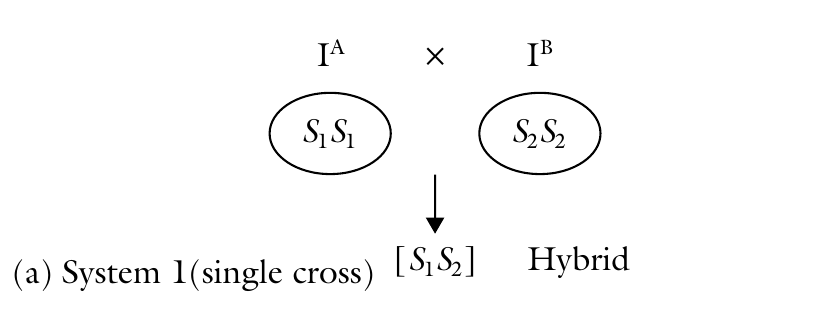
\includegraphics[width=0.5\linewidth]{./images/incompatibility_use_SC} 

}

\caption{Application of self-incompatibility in practical plant breeding (A)}\label{fig:si-use-sc}
\end{figure}
\end{frame}

\begin{frame}{}
\protect\hypertarget{section-9}{}
\begin{figure}

{\centering 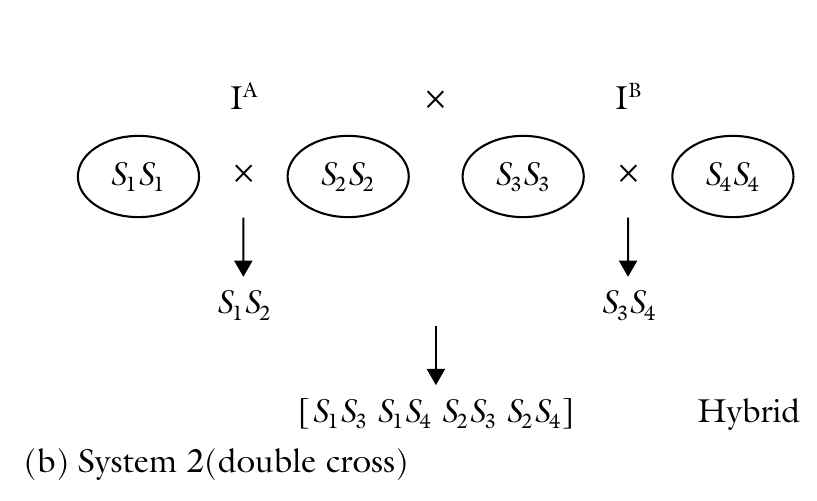
\includegraphics[width=0.5\linewidth]{./images/incompatibility_use_DC} 

}

\caption{Application of self-incompatibility in practical plant breeding (B)}\label{fig:si-use-dc}
\end{figure}
\end{frame}

\begin{frame}{}
\protect\hypertarget{section-10}{}
\begin{figure}

{\centering 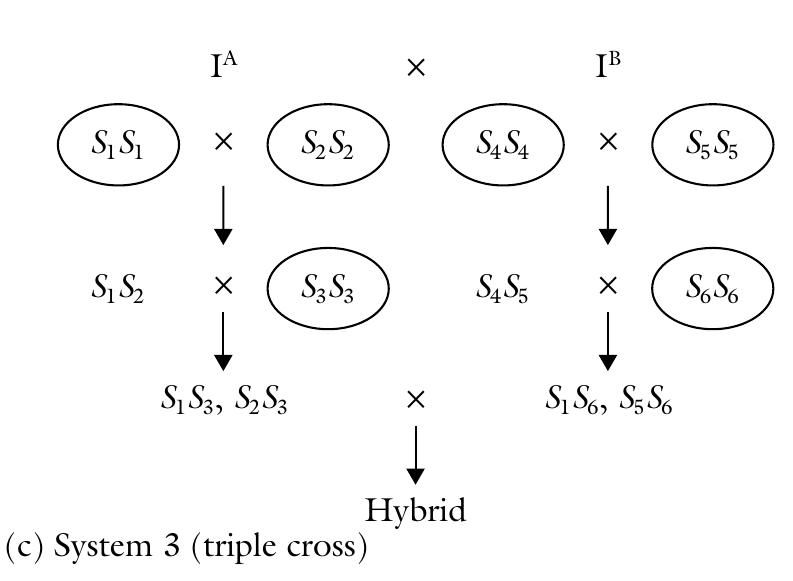
\includegraphics[width=0.5\linewidth]{./images/incompatibility_use_TC} 

}

\caption{Application of self-incompatibility in practical plant breeding (C)}\label{fig:si-use-tc}
\end{figure}
\end{frame}

\hypertarget{male-sterility}{%
\section{Male sterility}\label{male-sterility}}

\begin{frame}{}
\protect\hypertarget{section-11}{}
\begin{itemize}
\tightlist
\item
  Male sterility is a condition in plants whereby the anthers or pollen
  are non-functional. Male sterility also enforces cross-pollination.

  \begin{itemize}
  \tightlist
  \item
    as absence of or extreme scarcity of pollen,
  \item
    severe malformation or absence of flowers or stamens, or failure of
    pollen to dehisce.
  \item
    Similarly, it can be exploited as a tool to eliminate the need for
    emasculation for producing hybrid seed.
  \end{itemize}
\end{itemize}
\end{frame}

\begin{frame}{Kinds of sterility based on the origin of the abnormality}
\protect\hypertarget{kinds-of-sterility-based-on-the-origin-of-the-abnormality}{}
\begin{enumerate}
\tightlist
\item
  True male sterility - This is due to unisexual flowers that lack male
  sex organs (dioecy and monoecy), or bisexual flowers with abnormal or
  non-functional microspores (leading to pollen abortion).
\item
  Functional male sterility - The anthers fail to release their contents
  even though the pollen is fertile.
\item
  Induced male sterility - Plant breeders may use chemicals to induce
  sterility.
\end{enumerate}
\end{frame}

\begin{frame}{Genetic male sterility}
\protect\hypertarget{genetic-male-sterility}{}
\begin{itemize}
\tightlist
\item
  Genetic (nuclear, genic) male sterility is widespread in plants. The
  gene for sterility has been found in species including barley, cotton,
  soybean, tomato, potato, and lima bean.
\item
  It is believed that nearly all diploid and polyploidy plant species
  have at least one male sterility locus.
\item
  May be manifested as pollen abortion (pistillody) or abnormal anther
  development.
\item
  Genetic male sterility is often conditioned by a single recessive
  nuclear gene, \emph{ms}, the dominant allele, \emph{Ms}, conditioning
  normal anther and pollen development.
\item
  In alfalfa, however, two independently inherited genes have been
  reported
\item
  The expression of the gene may vary with the environment. But to be
  useful, the system must be stable
\end{itemize}
\end{frame}

\begin{frame}{Maintainance of GMS system}
\protect\hypertarget{maintainance-of-gms-system}{}
\begin{itemize}
\tightlist
\item
  The breeder cannot produce and maintain a pure population of male
  sterile plants.
\item
  The genetically male sterile types ( \emph{msms}) can be propagated by
  crossing them with a heterozygous pollen source ( \emph{Msms}).

  \begin{itemize}
  \tightlist
  \item
    What is the result of cross ?
  \end{itemize}
\item
  Breeders will always harvest 50\% male sterile plants by harvesting
  only the male sterile plants.
\item
  How to identify sterile from non sterile ?

  \begin{itemize}
  \tightlist
  \item
    Bright green hypocotyls in broccoli, leaf shape of potato and green
    stem in tomato
  \end{itemize}
\end{itemize}
\end{frame}

\begin{frame}{}
\protect\hypertarget{section-12}{}
\begin{figure}

{\centering 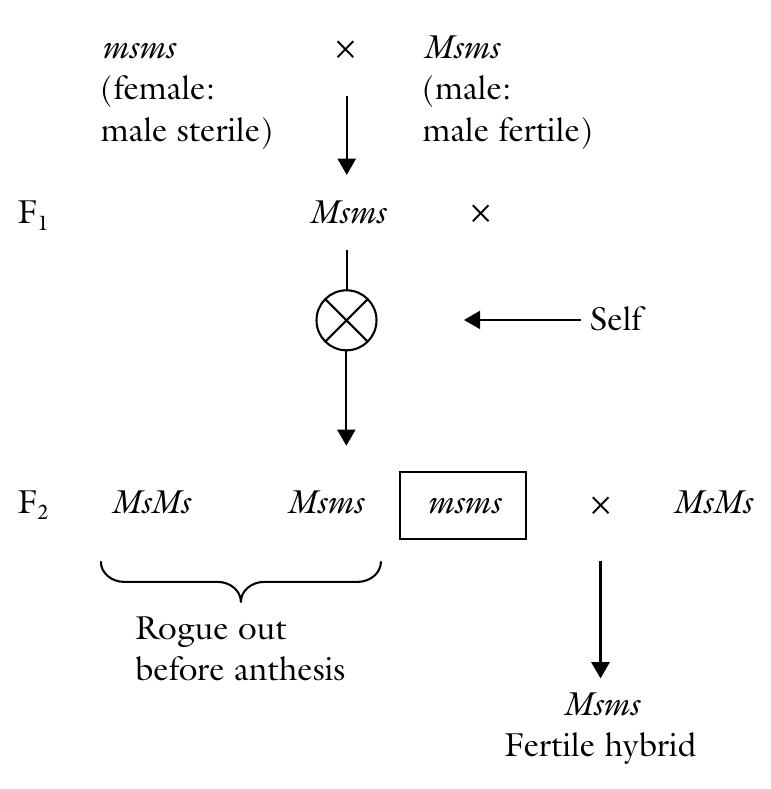
\includegraphics[width=0.5\linewidth]{./images/gms_use} 

}

\caption{Genetic male sterility as used in practical breeding}\label{fig:gms-use}
\end{figure}
\end{frame}

\begin{frame}{Cytoplasmic male sterility}
\protect\hypertarget{cytoplasmic-male-sterility}{}
\begin{itemize}
\tightlist
\item
  Sometimes, male sterility is controlled by the cytoplasm
  (mitochondrial gene) but may be influenced by nuclear genes.
\item
  A cytoplasm without sterility genes is described as normal (N)
  cytoplasm, while a cytoplasm that causes male sterility is called a
  sterile ( \emph{s}) cytoplasm or said to have cytoplasmic male
  sterility (CMS).
\item
  Transmitted through the egg only (maternal factor).
\item
  Has been found in species including corn, sorghum, sugar beet, carrot,
  and flax.
\item
  The condition has been induced in species such as sorghum by
  transferring nuclear chromosomes into a foreign cytoplasm.
\item
  Has real advantages in breeding ornamental species because all the
  offspring is male sterile, hence allowing them to remain fruitless.
\end{itemize}
\end{frame}

\begin{frame}{}
\protect\hypertarget{section-13}{}
\begin{figure}

{\centering 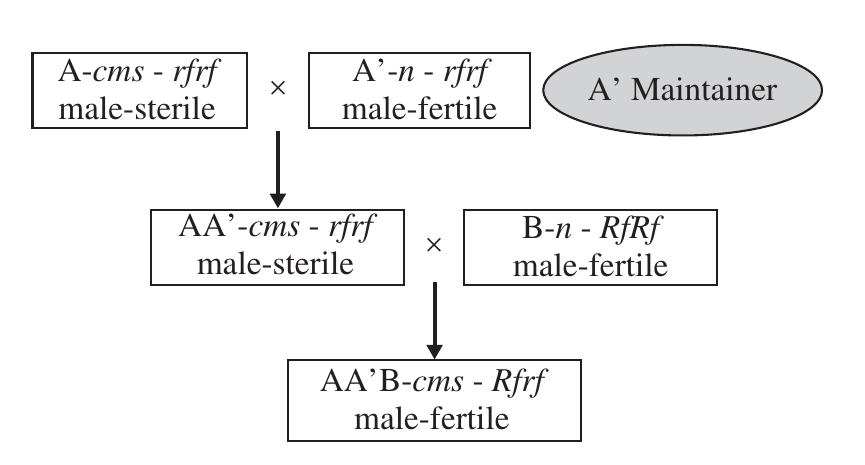
\includegraphics[width=0.5\linewidth]{./images/cms_use} 

}

\caption{Cytoplasmic male sterility as applied in plant breeding (N, normal cytoplasm; s, sterile cytoplasm).}\label{fig:cms-use}
\end{figure}
\end{frame}

\begin{frame}{}
\protect\hypertarget{section-14}{}
\begin{itemize}
\tightlist
\item
  Hybrid seed production using CMS requires three types of genotypes; -
  male fertile lines (called \emph{B} lines; maintained by selfing) with
  no cytoplasmic male sterility genes and which are homozygous for a
  dominant restorer gene (i.e.~normal ( \emph{n}) cytoplasm,
  \emph{RfRf});

  \begin{itemize}
  \tightlist
  \item
    cytoplasmic sterile female lines with male sterile cytoplasm but
    with no restorer genes (called \emph{A} lines; maintained by
    crossing with isogeneic cytoplasmic male fertile line);
  \item
    `male-fertile' female lines (called \emph{A'} lines or \emph{A'}
    maintainer lines; maintained by selfing) with normal cytoplasm and
    no restorer genes.
  \end{itemize}
\end{itemize}
\end{frame}

\begin{frame}{Cytoplasmic-genetic male sterility}
\protect\hypertarget{cytoplasmic-genetic-male-sterility}{}
\begin{itemize}
\tightlist
\item
  Cytoplasmic male sterility may be modified by the presence of
  fertility-restoring genes in the nucleus.
\item
  CMS is rendered ineffective when the dominant allele for the
  fertility-restoring gene ( \emph{Rf}) occurs, making the anthers able
  to produce normal pollen.
\item
  CMS is transmitted only through the egg, but fertility can be restored
  by \emph{Rf} genes in the nucleus.
\item
  Three kinds of progeny are possible following a cross, depending on
  the genotype of the pollen source.
\item
  The resulting progenies assume that the fertility gene will be
  responsible for fertility restoration.
\end{itemize}
\end{frame}

\begin{frame}{}
\protect\hypertarget{section-15}{}
\begin{figure}

{\centering 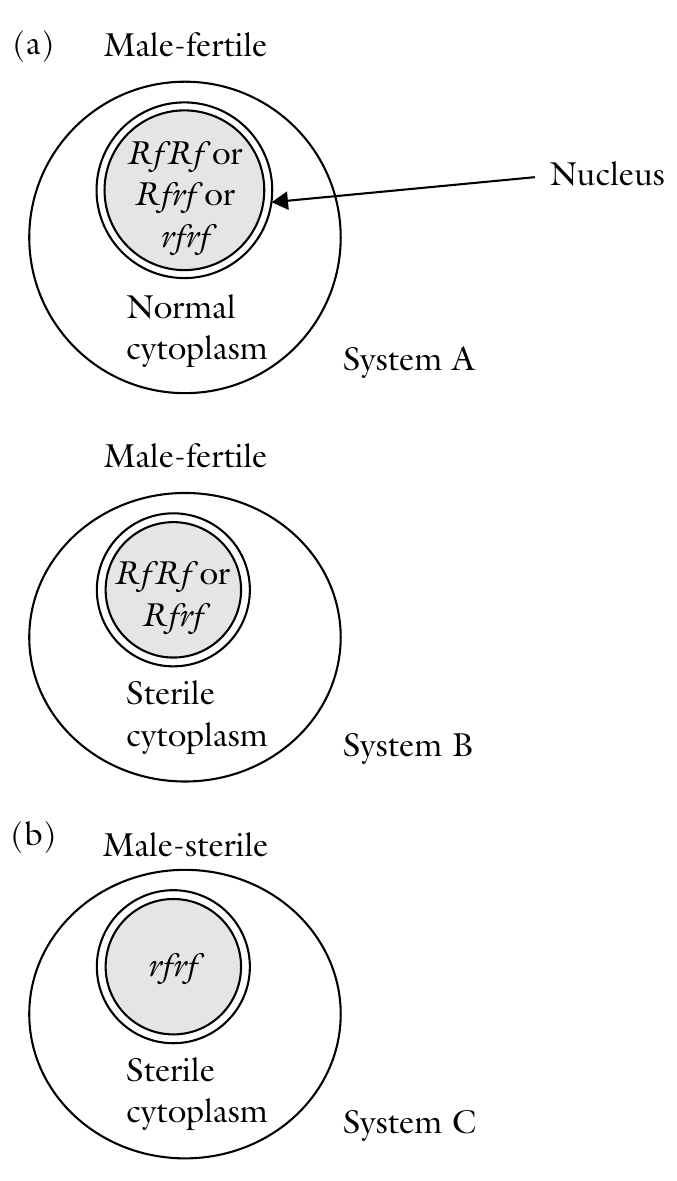
\includegraphics[width=0.3\linewidth]{./images/cgms_systems} 

}

\caption{The three systems of cytoplasmic genetic male sterility. The three factors involved in CMS are the normal cytoplasm (N), the male sterile cytoplasm (S), and the fertility restorer (Rf, rf).}\label{fig:cgms-systems}
\end{figure}
\end{frame}

\begin{frame}{Dichogamy (mechanism enforcing cross pollination)}
\protect\hypertarget{dichogamy-mechanism-enforcing-cross-pollination}{}
\begin{itemize}
\tightlist
\item
  Dichogamy is the maturing of pistils and stamens of a flower at
  different times.

  \begin{itemize}
  \tightlist
  \item
    Protogyny (stigma is receptive before the anther is mature to
    release the pollen)
  \item
    Protandry (pollen is released from the anther before the female is
    receptive).
  \end{itemize}
\end{itemize}
\end{frame}

\hypertarget{asexual-reproduction}{%
\section{Asexual reproduction}\label{asexual-reproduction}}

\begin{frame}{}
\protect\hypertarget{section-16}{}
\begin{itemize}
\tightlist
\item
  Production of offsprings that are genetically identical to the mother
  plant, and plants that are produced this way are called \emph{clones}.
\item
  Two methods of asexual reproduction

  \begin{itemize}
  \tightlist
  \item
    Reproduction through plant parts
  \item
    Reproduction through apomixis
  \end{itemize}
\end{itemize}
\end{frame}

\begin{frame}{Reproduction through plant parts}
\protect\hypertarget{reproduction-through-plant-parts}{}
\begin{itemize}
\tightlist
\item
  A \emph{bulb} is a modified shoot consisting of a very much shortened
  stem enclosed by fleshy leaves (e.g.~a tulip or an onion).
\item
  A \emph{corm} is a swollen stem base bearing buds in the axils of
  scale-like remains of leaves from the previous year's growth
  (e.g.~gladiolus).
\item
  A \emph{cutting} is an artificially detached part of a plant used as a
  means of vegetative propagation.
\item
  A \emph{rhizome} is an underground stem with buds in the axils of
  reduced leaves (e.g.~mint or couch grass).
\item
  A \emph{stolon} is a horizontally growing stem that roots at nodes
  (e.g.~strawberry runners).
\item
  A \emph{tuber} is a swollen stem that grows beneath the soil surface
  bearing buds (e.g.~potato).
\end{itemize}
\end{frame}

\begin{frame}{Reproduction by apomixis}
\protect\hypertarget{reproduction-by-apomixis}{}
\begin{itemize}
\tightlist
\item
  Asexual production of plant seeds can occur in obligate and
  facultative apomicts.
\item
  In facultative apomicts most seeds are asexually produced, since
  sexual reproduction can occur.
\item
  Apomixis arises by following mechanisms (based on which cells are
  responsible for producing an embryo)

  \begin{itemize}
  \tightlist
  \item
    Androgenesis (from the sperm nucleus of a pollen grain)
  \item
    Apospory (from somatic ovary cells)
  \item
    Diplospory (from 2n megaspore mother cell)
  \item
    Parthenogenesis (Egg cell without fertilization)
  \end{itemize}
\item
  In many cases, pollination must occur (pseudogamy) if viable apomictic
  seeds are to be formed.
\end{itemize}
\end{frame}

\hypertarget{reproductive-options-in-plants}{%
\section{Reproductive options in
plants}\label{reproductive-options-in-plants}}

\begin{frame}{Hermaphrodity versus unisexuality}
\protect\hypertarget{hermaphrodity-versus-unisexuality}{}
\begin{itemize}
\tightlist
\item
  Hermaphrodites have both male and female sexual organs, and hence may
  be capable of self fertilization. On the other hand, unisexuals,
  having one kind of sexual organ, are compelled to cross-fertilize.
  Each mode of reproduction has genetic consequences. Hermaphrodity
  promotes a reduction in genetic variability, whereas unisexuality,
  through cross-fertilization, promotes genetic variability.
\end{itemize}
\end{frame}

\begin{frame}{Self-pollination versus cross-pollination}
\protect\hypertarget{self-pollination-versus-cross-pollination}{}
\begin{itemize}
\tightlist
\item
  Hermaphrodites that are self-fertile may be self pollinated or
  cross-pollinated. In terms of pollen donation, a species may be
  autogamous (pollen comes from the same flower - selfing) or allogamous
  (pollen comes from a different flower). There are finer differences in
  these types. For example, there may be differences between the time of
  pollen shed and stigma receptivity.
\end{itemize}
\end{frame}

\begin{frame}{Self-fertilization versus cross-fertilization}
\protect\hypertarget{self-fertilization-versus-cross-fertilization}{}
\begin{itemize}
\tightlist
\item
  Just because a flower is successfully pollinated does not necessarily
  mean fertilization would occur. The mechanism of self-incompatibility
  causes some species to reject pollen from their own flowers, thereby
  promoting outcrossing.
\end{itemize}
\end{frame}

\begin{frame}{Sexuality versus asexuality}
\protect\hypertarget{sexuality-versus-asexuality}{}
\begin{itemize}
\tightlist
\item
  Sexually reproducing species are capable of providing seed through
  sexual means. Asexuality manifests in one of two ways - vegetative
  reproduction (in which no seed is produced) or agamospermy (in which
  seed is produced).
\end{itemize}
\end{frame}

\hypertarget{alternation-of-generation-in-flowering-plants}{%
\section{Alternation of generation in flowering
plants}\label{alternation-of-generation-in-flowering-plants}}

\begin{frame}{}
\protect\hypertarget{section-17}{}
\begin{figure}

{\centering 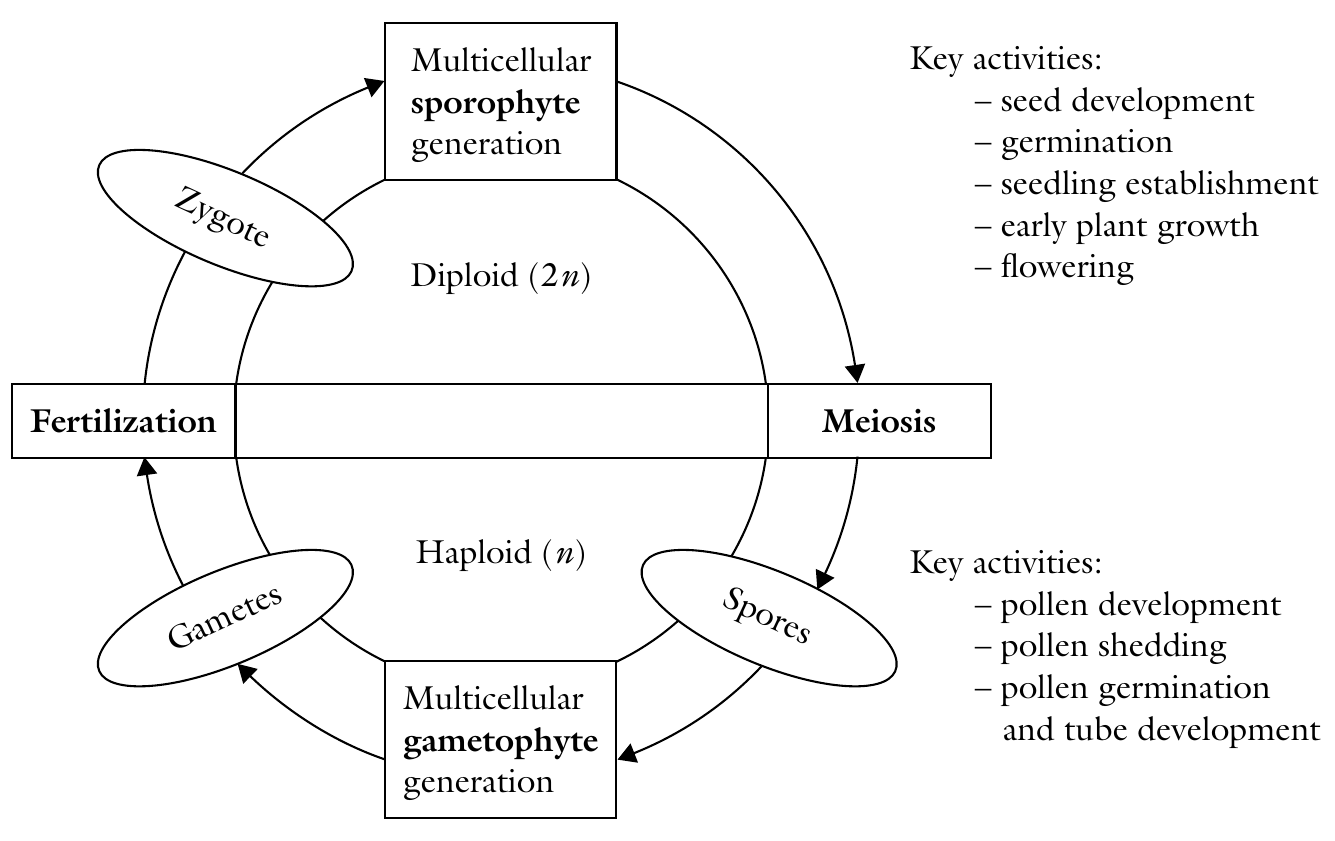
\includegraphics[width=0.6\linewidth]{./images/alternation_of_generations} 

}

\caption{Alternation of generations}\label{fig:alternation-generation}
\end{figure}
\end{frame}

\begin{frame}{}
\protect\hypertarget{section-18}{}
\begin{columns}[T,onlytextwidth]
  
  \column{0.5\linewidth}
  \footnotesize

\begin{figure}
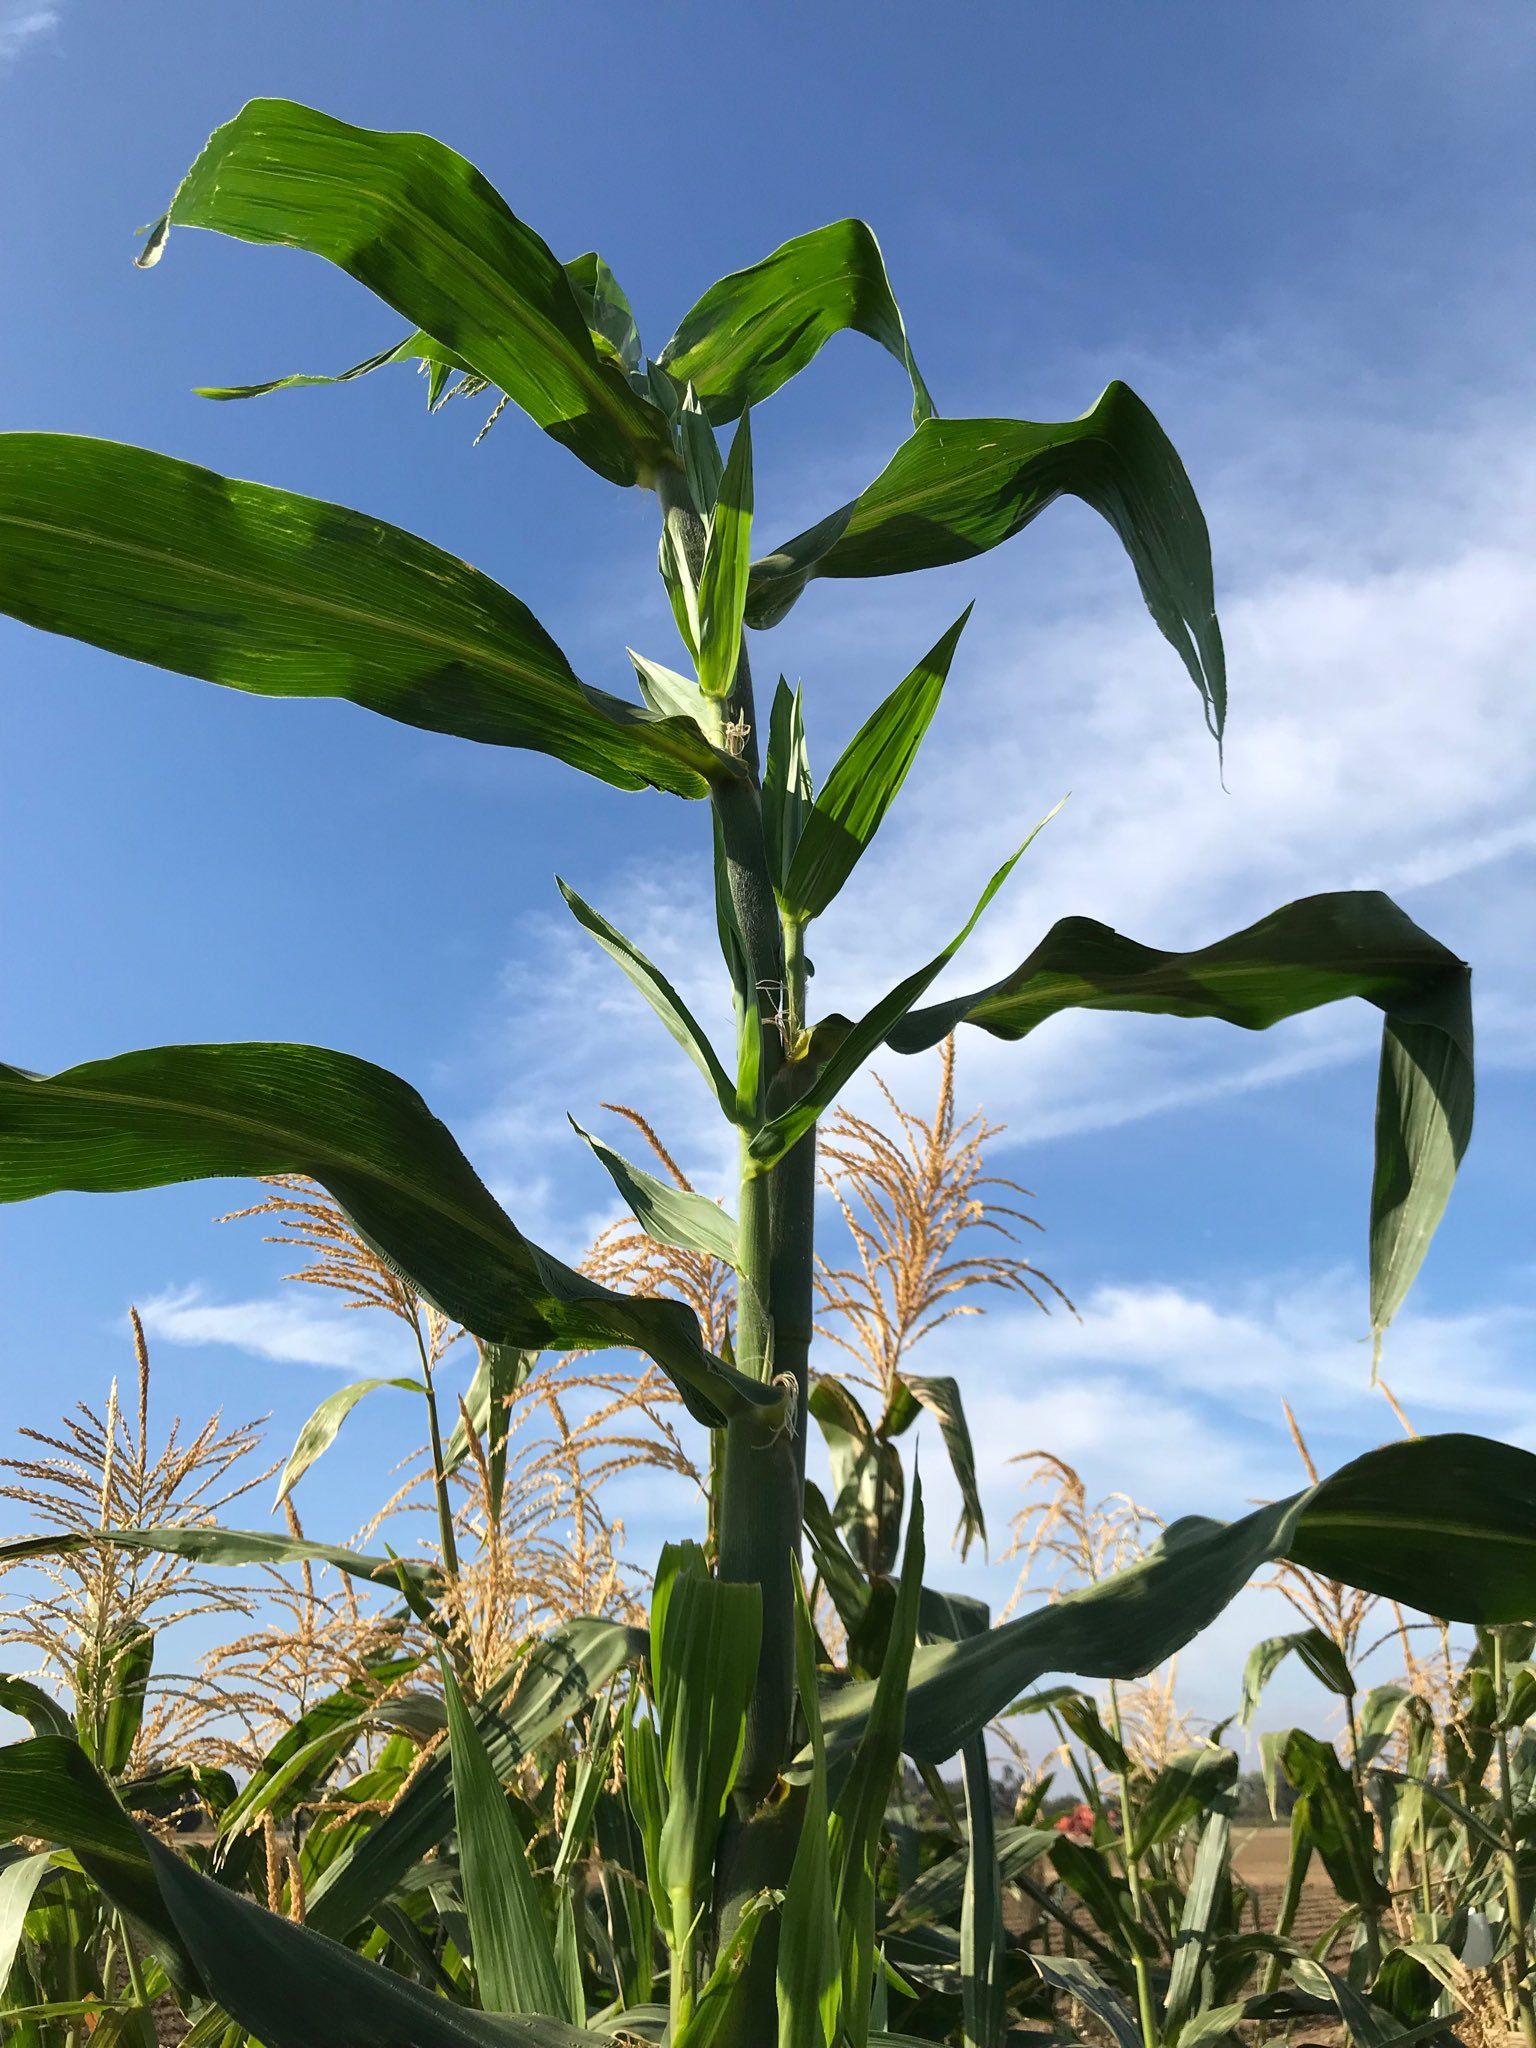
\includegraphics[width=0.6\linewidth]{./images/Teosinte_maize_hybrid_cross} \caption{Hybrid}\label{fig:hybrid}
\end{figure}

  \column{0.5\linewidth}
  \footnotesize
  
\begin{figure}
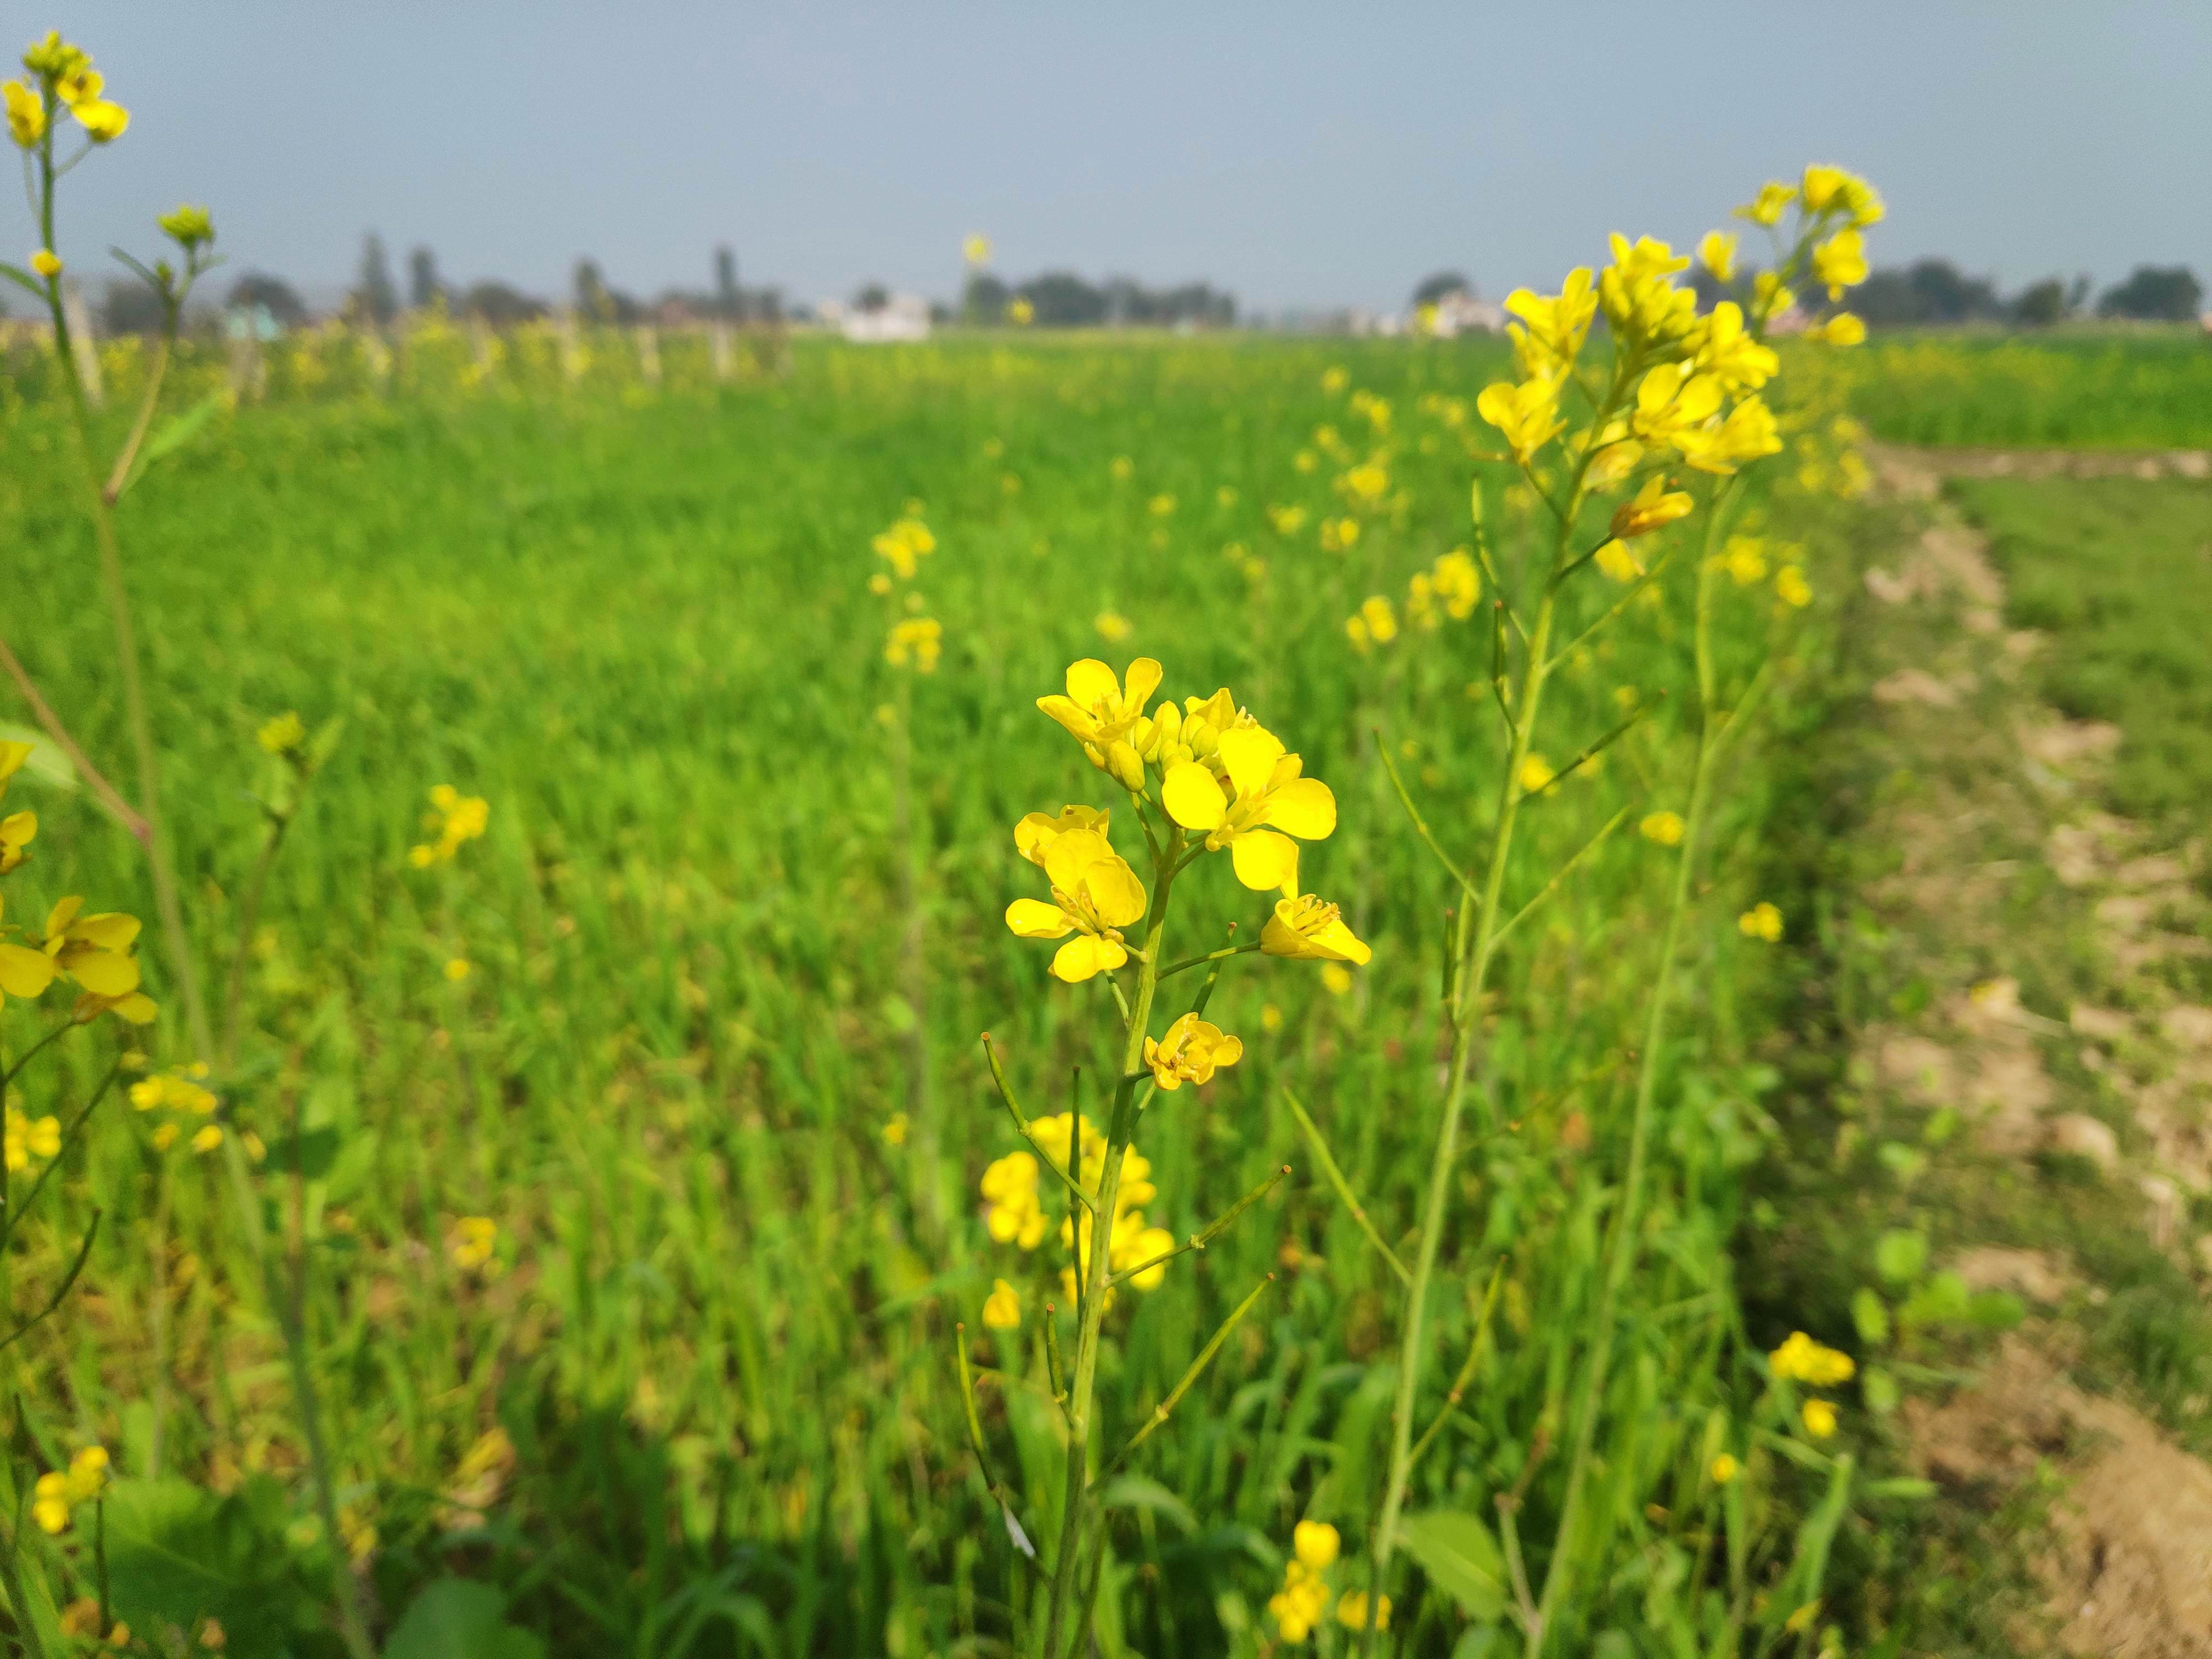
\includegraphics[width=0.8\linewidth]{./images/cross_pollinated_mustard} \caption{Open pollinated}\label{fig:openpollinated}
\end{figure}

\end{columns}
\end{frame}

\hypertarget{types-of-cultivar}{%
\section{Types of cultivar}\label{types-of-cultivar}}

\begin{frame}{}
\protect\hypertarget{section-19}{}
\begin{itemize}
\tightlist
\item
  Cultivar types include pure-lines, hybrids, clones, open-pollinated
  populations, composite-crosses, synthetics and multilines.
\item
  It is difficult, if not impossible to develop a pure-line cultivar of
  a crop species like potato ( \emph{Solanum tuberosum} ) as it is
  mainly reproduced vegetatively, and has many deleterious (or lethal)
  recessive alleles.
\item
  Similarly, pea ( \emph{Pisum sativum} ) is almost an obligate
  self-pollinator and so it would be difficult to develop hybrid pea, if
  nothing else seed production is likely to be expensive.
\end{itemize}
\end{frame}

\begin{frame}{Pure-line cultivars}
\protect\hypertarget{pure-line-cultivars}{}
\begin{itemize}
\tightlist
\item
  Pure-line cultivars are homozygous, or near-- homozygous, lines.
\item
  Can be produced most readily in naturally self-pollinating species.
\item
  It is generally accepted that it is normally one in which the line is
  homozygous for the vast majority of its loci (usually 90\% or more)
\item
  Commonly developed by inbreeding the species through continuous
  selfing of hybrid generated from crossing for 6-7 generations to the
  point where line is considered to be ``commercially true breeding''
\item
  Alternatively, doubled haploid lines may to generated
\end{itemize}
\end{frame}

\begin{frame}{}
\protect\hypertarget{section-20}{}
\begin{table}

\caption{\label{tab:predominantly-self-pollinated}Commonly self pollinated crops}
\centering
\fontsize{6}{8}\selectfont
\begin{tabular}[t]{ll}
\toprule
Common name & Scientific name\\
\midrule
Barley & \textit{Hordeum vulgare}\\
Chickpea & \textit{Cicer arietinum}\\
Clover & \textit{Trifolium spp.}\\
Common bean & \textit{Phaseolus vulgaris}\\
Cotton & \textit{Gossypium spp.}\\
\addlinespace
Cowpea & \textit{Vigna unguiculata}\\
Eggplant & \textit{Solanum melongena}\\
Flax & \textit{Linum usitatissimum}\\
Jute & \textit{Corchorus espularis}\\
Lettuce & \textit{Letuca sativa.}\\
\addlinespace
Oat & \textit{Avena sativa}\\
Pea & \textit{Pisum sativum}\\
Peach & \textit{Prunus persica}\\
Peanut & \textit{Arachis hypogaea}\\
Rice & \textit{Oryza sativa}\\
\addlinespace
Sorghum & \textit{Sorghum bicolor}\\
Soybean & \textit{Glycine max}\\
Tobacco & \textit{Nicotiana tabacum}\\
Tomato & \textit{Solanum lycopersicum}\\
Wheat & \textit{Triticum aestivum}\\
\bottomrule
\end{tabular}
\end{table}
\end{frame}

\begin{frame}{Open pollinated cultivars}
\protect\hypertarget{open-pollinated-cultivars}{}
\begin{itemize}
\tightlist
\item
  Heterogenous populations comprised of different plants which are
  genetically non-identical.
\item
  Also heterozygous
\item
  Almost exclusively from cross pollinating species
\item
  Stable for character of interest
\item
  e.g.: Onions, rye, herbage grass, non-hybrid sweetcorn, sugar beet and
  oil palm
\end{itemize}

\begin{figure}

{\centering 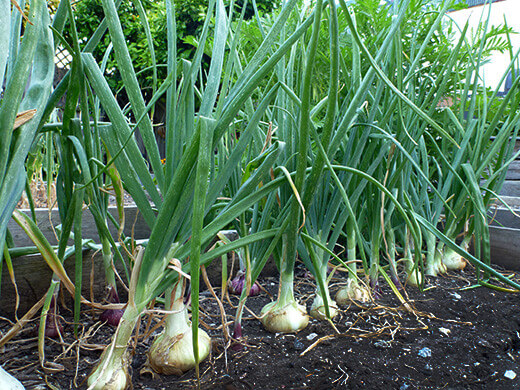
\includegraphics[width=0.35\linewidth]{./images/open_pollinated_onion} 

}

\caption{Open pollinated crops}\label{fig:unnamed-chunk-1}
\end{figure}
\end{frame}

\begin{frame}{Hybrid}
\protect\hypertarget{hybrid}{}
\begin{itemize}
\tightlist
\item
  Hybrid cultivars have different leves of homogeneity but, importantly
  are highly heterozygous.
\item
  Exploits the phenomenon of heterosis
\item
  Variants exist:

  \begin{itemize}
  \tightlist
  \item
    Single cross
  \item
    Double cross
  \item
    Three way cross
  \end{itemize}
\item
  Is one of the most complex of breeding methods

  \begin{itemize}
  \tightlist
  \item
    Inbred line development
  \item
    Test cross comparison
  \item
    Selection and hybridization
  \end{itemize}
\end{itemize}
\end{frame}

\begin{frame}{Clonal cultivars}
\protect\hypertarget{clonal-cultivars}{}
\begin{itemize}
\tightlist
\item
  Clonal cultivars are genetically uniform but tend to be highly
  heterozygous
\item
  Uniformity of plant types is maintained through vegetative rather than
  sexual reproduction.
\item
  Cultivars are vegetatively propagated by asexual reproduction
  (cloning) including

  \begin{itemize}
  \tightlist
  \item
    cuttings,
  \item
    tubers,
  \item
    bulbs,
  \item
    rhizomes,
  \item
    grafts
  \end{itemize}
\item
  A cultivar can also be classified as a clone if it is propagated
  through obligate apomixis (e.g.~buffelgrass)
\item
  Genetic constitution of cloned selection remains `fixed'
\item
  e.g.: Potatoes, Bananas, Peaches, Apples, Cassava, Sugarcane,
  Strawberries, Blueberries and Chrysanthemums.
\end{itemize}
\end{frame}




\end{document}
